%%
%% This is file `sample-sigconf.tex',
%% generated with the docstrip utility.
%%
%% The original source files were:
%%
%% samples.dtx  (with options: `sigconf')
%% 
%% IMPORTANT NOTICE:
%% 
%% For the copyright see the source file.
%% 
%% Any modified versions of this file must be renamed
%% with new filenames distinct from sample-sigconf.tex.
%% 
%% For distribution of the original source see the terms
%% for copying and modification in the file samples.dtx.
%% 
%% This generated file may be distributed as long as the
%% original source files, as listed above, are part of the
%% same distribution. (The sources need not necessarily be
%% in the same archive or directory.)
%%
%%
%% Commands for TeXCount
%TC:macro \cite [option:text,text]
%TC:macro \citep [option:text,text]
%TC:macro \citet [option:text,text]
%TC:envir table 0 1
%TC:envir table* 0 1
%TC:envir tabular [ignore] word
%TC:envir displaymath 0 word
%TC:envir math 0 word
%TC:envir comment 0 0
%%
%%
%% The first command in your LaTeX source must be the \documentclass
%% command.
%%
%% For submission and review of your manuscript please change the
%% command to \documentclass[manuscript, screen, review]{acmart}.
%%
%% When submitting camera ready or to TAPS, please change the command
%% to \documentclass[sigconf]{acmart} or whichever template is required
%% for your publication.
%%
%%
\documentclass[sigconf]{acmart}
\settopmatter{printacmref=false} % Removes citation information below abstract
\renewcommand\footnotetextcopyrightpermission[1]{} % removes footnote with conference information in first column
\pagestyle{plain} % removes running headers


\usepackage{hyperref}
\usepackage{graphicx}
\usepackage{ulem}
\usepackage{listings}
\usepackage{xcolor}


%%
%% \BibTeX command to typeset BibTeX logo in the docs
\AtBeginDocument{%
  \providecommand\BibTeX{{%
    Bib\TeX}}}




%%
%% end of the preamble, start of the body of the document source.
\begin{document}

%%
%% The "title" command has an optional parameter,
%% allowing the author to define a "short title" to be used in page headers.
\title{Exploring Parallelism Opportunities in KLayout (project proposal, group 23)}

%%
%% The "author" command and its associated commands are used to define
%% the authors and their affiliations.
%% Of note is the shared affiliation of the first two authors, and the
%% "authornote" and "authornotemark" commands
%% used to denote shared contribution to the research.
\author{Zeren Chen}
\authornote{Still trying to reach out to teammate}
\email{TBD@TBD.tw}
\affiliation{%
  \institution{}
  \country{Taiwan}
}

\author{MH Yan }
\email{TBD@TBD.tw}
\affiliation{%
  \institution{}
  \country{Taiwan}
}

\author{ChatGpt}
\affiliation{%
  \institution{Open AI }
  \country{USA}
}


%%
%% By default, the full list of authors will be used in the page
%% headers. Often, this list is too long, and will overlap
%% other information printed in the page headers. This command allows
%% the author to define a more concise list
%% of authors' names for this purpose.
\renewcommand{\shortauthors}{Zeren et al.}

% %%
% %% The abstract is a short summary of the work to be presented in the
% %% article.
% \begin{abstract}
%   A clear and well-documented \LaTeX\ document is presented as an
%   article formatted for publication by ACM in a conference proceedings
%   or journal publication. Based on the ``acmart'' document class, this
%   article presents and explains many of the common variations, as well
%   as many of the formatting elements an author may use in the
%   preparation of the documentation of their work.
% \end{abstract}

%%
%% Keywords. The author(s) should pick words that accurately describe
%% the work being presented. Separate the keywords with commas.
\keywords{ KLayout, DRC, Parallel Programming, Open-Source}
%% A "teaser" image appears between the author and affiliation
%% information and the body of the document, and typically spans the
%% page.
% \begin{teaserfigure}
%   \includegraphics[width=\textwidth]{sampleteaser}
%   \caption{Seattle Mariners at Spring Training, 2010.}
%   \Description{Enjoying the baseball game from the third-base
%   seats. Ichiro Suzuki preparing to bat.}
%   \label{fig:teaser}
% \end{teaserfigure}

% \received{20 February 2007}
% \received[revised]{12 March 2009}
% \received[accepted]{5 June 2009}

%%
%% This command processes the author and affiliation and title
%% information and builds the first part of the formatted document.
\maketitle

\section{Introduction}
Design Rule Checking (DRC) is a crucial step in the VLSI design process, ensuring that the layout adheres to the specified design rules. Some basic and common types of DRC rules are:

\begin{itemize}
\item Minimum width
\item Minimum spacing 
\item Minimum area 
\end{itemize}


\begin{figure}[h]
  \centering
  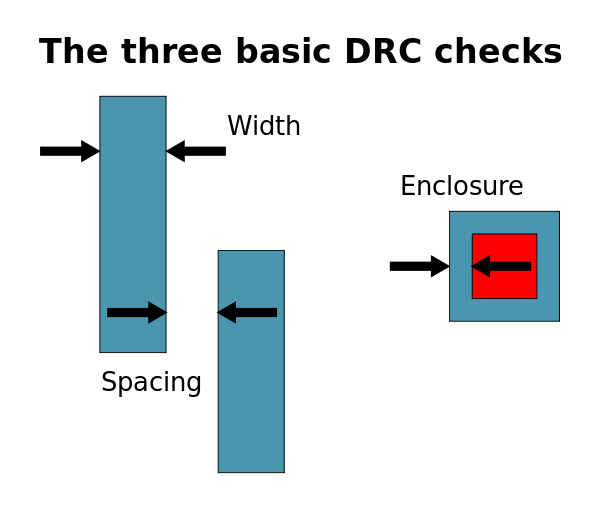
\includegraphics[width=0.4\textwidth]{600px-The_three_basic_DRC_checks.png}
  \caption{The three basic DRC checks (source: \href{https://upload.wikimedia.org/wikipedia/commons/thumb/5/5a/The_three_basic_DRC_checks.svg/600px-The_three_basic_DRC_checks.svg.png}{Wikipedia})}
  \label{fig:basic_drc_checks}
\end{figure}

KLayout(\href{https://www.klayout.de/}{https://www.klayout.de}), an open-source layout viewer and editor, is widely used for VLSI design, including DRC feature support. However, as the complexity of IC designs increases, the computational demands of KLayout's DRC also increase. This project aims to learn how DRC works in Klayout, explore opportunities for parallelism within KLayout using threading, SIMD techniques, and advanced parallel programming techniques such as OpenMP, MPI, and CUDA, if time permits. Additionally, we will analyze the DRC run set written in Python to find the possibility of task parallelism. Furthermore, we will attempt to reach out to the KLayout author to gather valuable feedback and insights to guide our project.


\section{Statement of the problem}
The primary focus of this project is to identify areas within KLayout's DRC where parallelism can be applied to improve its performance, particularly in terms of processing large and complex layout designs. To achieve this, we will analyze the existing KLayout codebase, focusing on the DRC run set written in Python/Ruby, and identify bottlenecks and opportunities for parallelization, including task parallelism, in the DRC process.

\lstset{
  basicstyle=\ttfamily,
  frame=single,
  breaklines=true,
  keywordstyle=\color{blue!70},
  commentstyle=\color{green!70},
  stringstyle=\color{red!70},
  numbers=left,
  numberstyle=\tiny,
  numbersep=5pt,
  tabsize=2
}

\begin{lstlisting}[language=Ruby, caption=Sample DRC code in KLayout, label=lst:sample_drc_code]
  report("A simple script")

  active = input(1, 0)
  poly = input(6, 0)
  gate = active & poly
  gate.width(0.3).output("gate_width", "Gate width violations")
  
  metal1 = input(17, 0)
  metal1.width(0.7).output("m1_width", "M1 width violations")
  metal1.space(0.4).output("m1_space", "M1 spacing violations")
  
  
\end{lstlisting}
This script will compute the gate poly shapes from the active and poly layers using a boolean "AND". The active layer has GDS layer 1, while the poly layer has GDS layer 6. On this computed gate layer, the script will perform a width check for 0.3 micrometer. In addition a width and space check is performed on the first metal layer, which is on GDS layer 17. 


\section{Proposed approaches}
We will first conduct a detailed code analysis of KLayout's DRC, focusing on the Python/Ruby run set, to identify computationally intensive tasks and potential areas for parallelization. 
For example, C++ code that implements width, space operations of Listing \ref{lst:sample_drc_code}.  Next, we will design and implement a parallelized version of KLayout's DRC using threading techniques (e.g., Pthreads, OpenMP) and SIMD (Single Instruction, Multiple Data) instructions. If time permits, we will also explore the possibility of employing advanced parallel programming techniques such as MPI and CUDA learned in the class. We will then evaluate the performance of the parallelized DRC by measuring the time taken to process various layout designs generated by scripts written by us or some real open source CMOS designs available. 


\section{Language selection}
Ideally, we would like to apply all the techniques learned in the class to improve the run time of certain DRC C++ code called by DRC runset written in Python/Ruby.
\begin{itemize}
  \item SIMD
  \item Threading 
  \item OpenMP 
  \item MPI(less likely as klayout only works on single host)
  \item CUDA
\end{itemize}
We will also explore the possibility of using the \href{https://taskflow.github.io/}{Taskflow} library, a modern C++ parallel and heterogeneous task programming library, to achieve parallelism in KLayout's DRC.

\section{Related work}
A preliminary literature search indicates limited research on parallelization opportunities within KLayout's DRC. As a result, our project will provide valuable insights into improving the performance of KLayout's DRC and contribute to the growing body of knowledge in the field.

\section{Statement of expected results}
Our primary focus is on learning and gaining experience working with large codebases and open-source communities. We expect to identify potential areas for parallelization within KLayout's DRC, including task parallelism, and attempt to implement a parallelized version using threading, SIMD techniques, and advanced parallel programming techniques (if time permits). Although our work may not be accepted upstream, we aim to demonstrate improved performance in terms of processing time for large and complex layout designs, and to acquire valuable insights and practical knowledge through our exploration of KLayout's DRC.

\section{Tentative Timetable}
\begin{itemize}
    \item April 7 - May 31, 2023: 
    \begin{itemize}
      \item Reviewing the source code of KLayout and find portions that can be parallelized.
      \item Prepare test run set, test cases, benchmarking serial versions.
      \item Work on threading, SIMD, openMP, CUDA, taskflow versions respectively.
    \end{itemize}
    \item June 1 - 15, 2023: Prepare final report and presentation slides
    \item June 16, 2023: Submit final report, source codes
\end{itemize}

\section{References}
\begin{itemize}
  \item KLayout Documentation, "KLayout User Manual," [Online]. Available: https://www.klayout.de/doc/index.html [Accessed: 04-April-2023].
  \item KLayout Repository, "KLayout Source Code," [Online]. Available: https://github.com/KLayout/klayout [Accessed: 04-April-2023].
  \item Taskflow, "Taskflow: A General-purpose Parallel and Heterogeneous Task Programming System," [Online]. Available: https://taskflow.github.io/ [Accessed: 04-April-2023].
\end{itemize}
\end{document}
\endinput
%%
%% End of file `sample-sigconf.tex'.
